\chapter{Design and Solution}

\section{System Structure}
Overall, the system includes three parts of hardware modules: a camera module, the user's smartphone, and the server.

Our sign language translating AI system includes six main modules: hand pattern recognition, direction determination, location detection, action detection, word decoder, and text to speech (Figure TK). Firstly, the system continuously captures the hand's motion, processes it with the hand landmark model, and then puts it into those modules. Each of them has a unique role, and after combining the first four modules' results (hand pattern, direction, location, and action detection), the word decoder module will take the output data and bring out the corresponding outcome. Then, the result will show up on the main screen (Figure TK); meanwhile, the phone will speak out that word. In the below sections, we will discuss each module's role and how it works.

TODO: Replace with new structure
TODO: Trình bày cả 2 mô hình, giới thiệu luôn action detection và nói là do không khả thi nên đề xuất mô hình mới, khi đó sẽ có sự thay đổi như thế nào 

\begin{figure}[H]
	\centering
	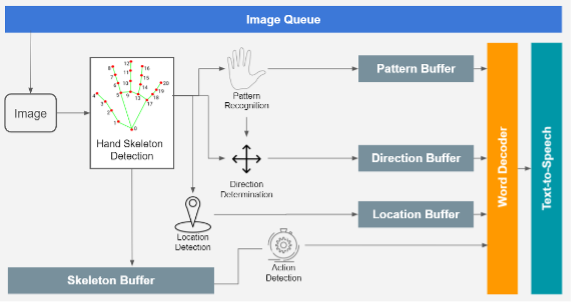
\includegraphics[width=\textwidth]{img/Chap4/OverviewOfTheSystemModules.png}
	\caption{Overview of the system modules}
	\label{fig:Chap4-OverviewOfTheSystemModules}
\end{figure}

\section{Detail Implementation}

\subsection{Hand pattern recognition}

Hand pattern recognition is the first and basic module of this system. While a person with disabilities does signs of sign language, his hands perform a series of different movements, where their hand may be spread out, clenched, or his fingers pointing out at something. Therefore, the role of this module is to recognize the pattern of the hands. Then combining the outcome with other modules, the system can give out the final result.

This module uses the output of the hand landmark model, which is a matrix size of 21. After calculating all the values in that matrix, we get a new matrix representing the distance between those 21 coordinates. Using the distance matrix as the input of CNN [TK] with the designed structure (see Figure \ref{fig:Chap4-StructureOfConvolutionalNeuralNetwork}), as seen in Figure \ref{fig:Chap4-OverviewOfTheSystemModules}, will tell us the pattern of the hand at the moment it is captured.

\begin{figure}[H]
	\centering
	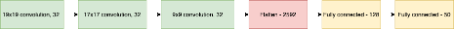
\includegraphics[width=\textwidth]{img/Chap4/StructureOfConvolutionalNeuralNetwork.png}
	\caption{Structure of convolutional neural network}
	\label{fig:Chap4-StructureOfConvolutionalNeuralNetwork}
\end{figure}

\subsection{Direction determination}
FIXME: Thêm các hình ảnh về cách xác định hướng, lấy từ ppt

The directions of the hand include four directions, i.e., right, left, up, down, front, and back. Each hand's pattern combined with different directions leads to a different meaning. For example, the pattern that points at someone means the word "you"; on the other hand, when we point at ourselves, it means the word I (see Figure \ref{fig:Chap4-WordYouInSignLanguage} and Figure \ref{fig:Chap4-WordIInSignLanguage}).

\begin{figure}[H]
	\centering
	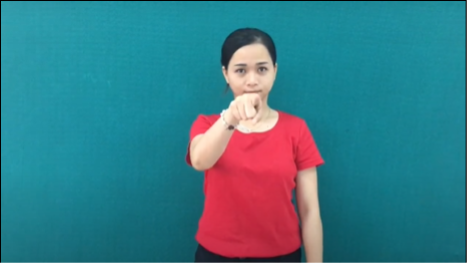
\includegraphics[width=\textwidth]{img/Chap4/WordYouInSignLanguage.png}
	\caption{Word "You" (bạn) in sign language}
	\label{fig:Chap4-WordYouInSignLanguage}
\end{figure}

\begin{figure}[H]
	\centering
	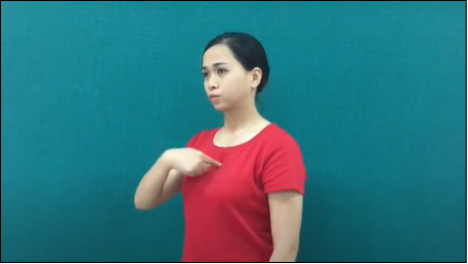
\includegraphics[width=\textwidth]{img/Chap4/WordIInSignLanguage.png}
	\caption{Word "I" (tôi) in sign language}
	\label{fig:Chap4-WordIInSignLanguage}
\end{figure}

To determine the hand's direction, we use the hand landmark model provided in MediaPipe (see section 2 TK). The inception here is that we calculate the distance between the tip of the index finger and the wrist (called TK), then project it to the axis Ox, Oy, Oz, respectively. After that, we take each of those coordinates and compare them with the others. Finally, the one with the immense value will tell which axis the hand is on; besides, with the direction from the wrist to the tip of the index finger projected on that corresponding axis, we will know which direction the hand is.

For instance, a hand is known to be pointing toward the left direction. The value of the distance, when projected on the axis Ox, will be the biggest one among the three projected values. Then, calculate the vector drawn from the wrist to the tip of the index finger; we will know the direction of the hand itself.

\subsection{Location detection}
FIXME: Giới thiệu previous approach về sử dụng độ zoom, các khó khăn
FIXME: Thêm các hình ảnh về cảm biến sóng âm, các thông số, tại sao lại sử dụng, sử dụng như thế nào

Locations of hand vary, is the hand put at forehead, mouth or the chest level, and so on. Every hand pattern that goes with every location will result in different words. Nevertheless, it is hard for the AI to know the hand's coordinates with only one camera, and its view is from above (see Figure \ref{fig:Chap4-ViewFromCamera}). However, we came up with some solutions to this issue.

Firstly, we will take pictures of the hand and calculate the size of the hand in every frame in order to know whether that hand is getting bigger or smaller. Hence, if that hand is smaller than before, it means the hand is getting far away from the camera, and its location is somewhere at the chest level or the stomach level.

\begin{figure}[H]
	\centering
	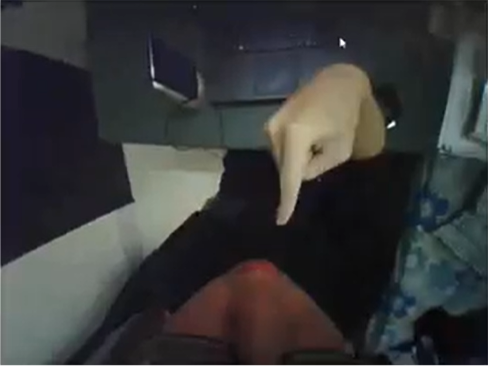
\includegraphics[width=\textwidth]{img/Chap4/ViewFromCamera.png}
	\caption{View from the camera module}
	\label{fig:Chap4-ViewFromCamera}
\end{figure}

Nonetheless, the above solution still has an issue: every man's hand has a different size, and the system does not know the correct position of the hand. Therefore, another solution is to use a wide-angle camera and set it away from the forehead. With this solution, the camera can have a much broader view. However, since we only have a normal-angle camera, we could not try out this solution and confirm its suitability.

\subsection{Design}
TODO: Trình bày các thiết kế hiện có và các chức năng phụ

\subsection{Word decoder}
% TODO:   Previous approach 

% [x] How to map word ?

% TODO:   New approach

% [x] Punish function

% [x] Using beam search

% [x] CTC decode

% [x] Flow

% [x] Expected result

% [...] Difficult and proposed solution

% [...] Dịch sang tiếng anh

% [...] Thêm các hình ảnh


% TODO: With previous approach

As discussed above, there are considerable technical difficulties in implementing the action detection module. We did some research and proposed a new model to resolve these problems. As a result, this change affects the word decoder module, which needs some adjustments.

The previous model decodes a word into four factors: pattern, location, direction, and action. After getting the outputs from the four modules, it will search the database to find the corresponding word. Figure \ref{fig:Chap4-MapWord} illustrates how an input containing four factors is mapped to the correct word in the database. Applying a basic searching algorithm, we have the system find the most appropriate word. If it can not find any, it will replace or deprecate some parts of the input and try again to find another word. After decoding and finding the suitable word, the application will display that word on the screen.

\begin{figure}[H]
	\centering
	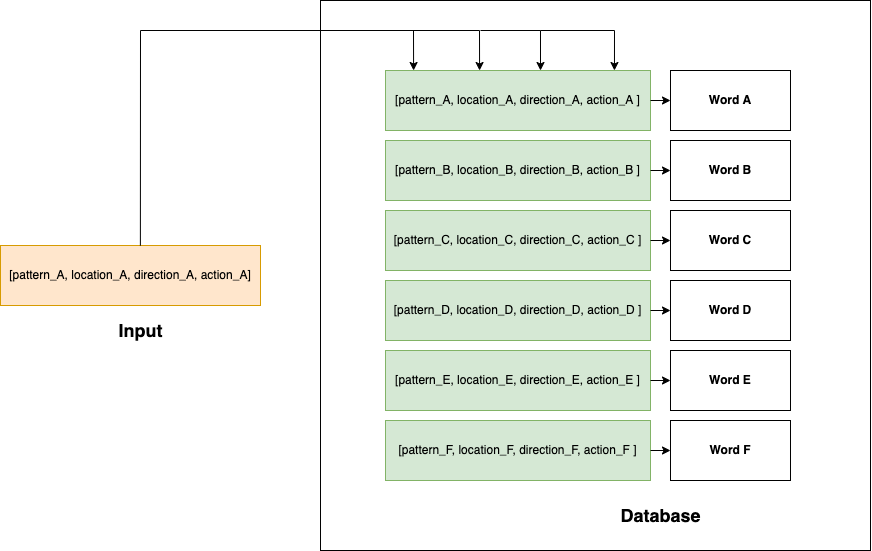
\includegraphics[width=\textwidth]{img/Chap4/MapWord.png}
	\caption{Map one to one data from four component with word in database and get result}
	\label{fig:Chap4-MapWord}
\end{figure}

\subsubsection{ Introduction to handstate }

Right after the deprecation of the action detection module, the question that comes up is how we can find the correct word without that module. Therefore, we propose a different model for a word that is not decoded into four factors like the previous model. It only contains three elements left: pattern, direction, and location. Consequently, each set of those three elements is called a hand state (\ref{fig:Chap4-HandState}), and a word is decoded into many different hand states.

This concept of hand state comes from the research of natural language processing, in which a word is composed of many characters. Accordingly, a word is concatenated from many hand states in this thesis. Then, we will get the desired word when going through the processing steps that we will discuss later in this proposal.

\begin{figure}[H]
  \centering
  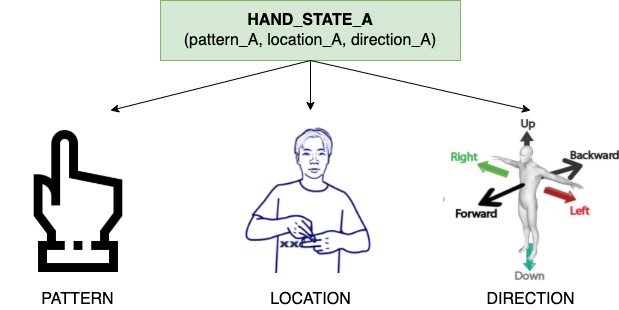
\includegraphics[width=0.6\textwidth]{img/Chap4/HandState.png}
  \caption{ Hand State which construct from pattern, location and direction}
  \label{fig:Chap4-HandState}
\end{figure}

\subsubsection{ Using beam search and CTC decode to map word}

After we have grasped the concept of hand state, we will come to the essential part of the model: converting the received hand states into words.
      
\begin{figure}[H]
  \centering
  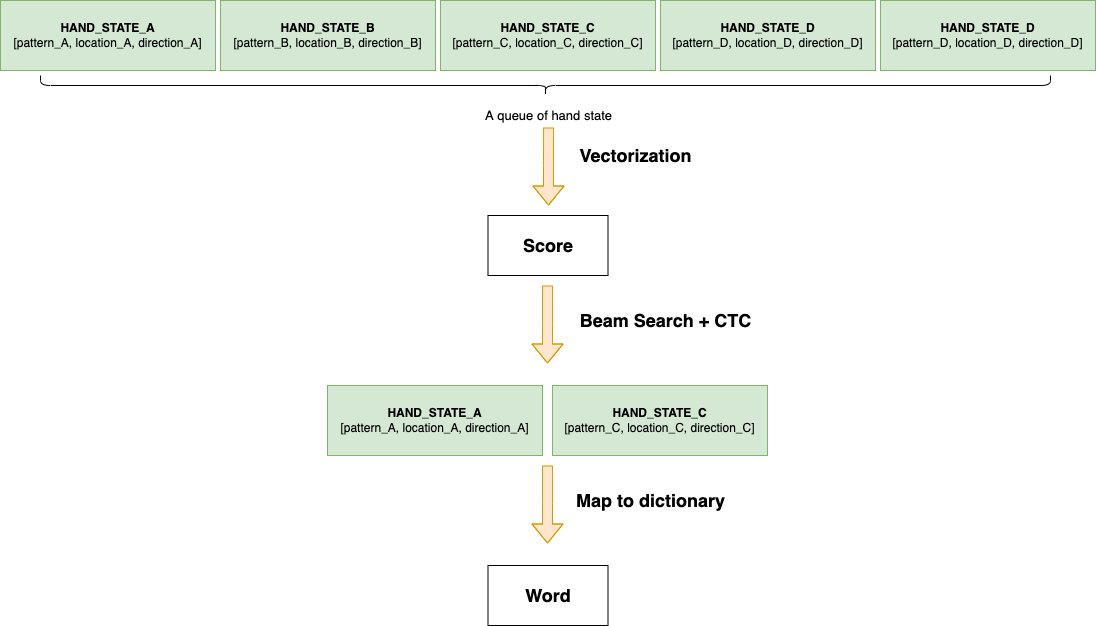
\includegraphics[width=\textwidth]{img/Chap4/Architechture.png}
  \caption{Architechture}
  \label{fig:Chap4-Architechture}
\end{figure}

Figure \ref{fig:Chap4-Architechture} is the model proposed by the authors for this section. The input will be a queue of hand states taken from the previous three components. Here, in our conventions, the queue length is set to 5, but it is not the final number, as we need more calculations and experimentation to find the right queue length. This model consists of three steps:

\begin{enumerate}
  \item \textbf{Vectorization:} This step converts a queue of many hand states \ref{fig:Chap4-HandStateQueue} into a matrix as input for beam search.
  \item \textbf{Beam search:} In this step, we will perform a beam search algorithm to choose which hand states are suitable for the input from the database. Besides, we propose using the CTC decode model to eliminate the wrong hand states or previous duplicated hand states, increasing the model's efficiency.
  \item \textbf{Map to the dictionary:} And finally, after going through the above two steps, from the initial queue, we will get the most likely hand states. Our job is to map these hand states to the database and find the correct word.
\end{enumerate}
      
\subsubsection{ Vectorization }
% TODO: Why we need punish
% TODO: how to perform -> Trình bày cách đánh giá như thế nào, cách trừ điểm và các phương châm đánh giá
% TODO: Sau khi punish dùng hàm softmax để chuyển các giá trị về dạng xác suất

When we get to this step, we get a queue of hand states. Because before entering the beam search module, we need a matrix representing the correlation between the outputs received from the components and the data in the database.

\begin{figure}[H]
  \centering
  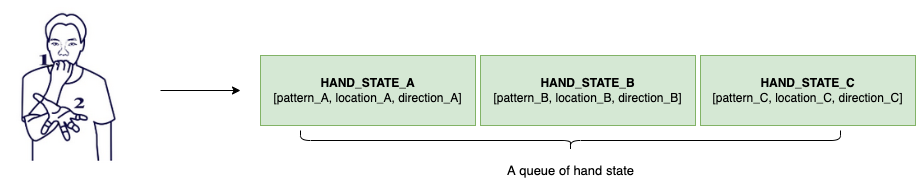
\includegraphics[width=\textwidth]{img/Chap4/HandStateQueue.png}
  \caption{A queue of hand state which get from three component in section ... }
  \label{fig:Chap4-HandStateQueue}
\end{figure}

From this queue, we will cycle through each hand state, compare it with the available hand state database, and evaluate the score for it based on the following principles \ref{fig:Chap4-Vectorization}:

\begin{enumerate}
  \item The score will be increased if the hand state matches the word in the database.
  \item Otherwise, the score will be decreased if that hand state does not match any.
\end{enumerate}

\begin{figure}[H]
  \centering
  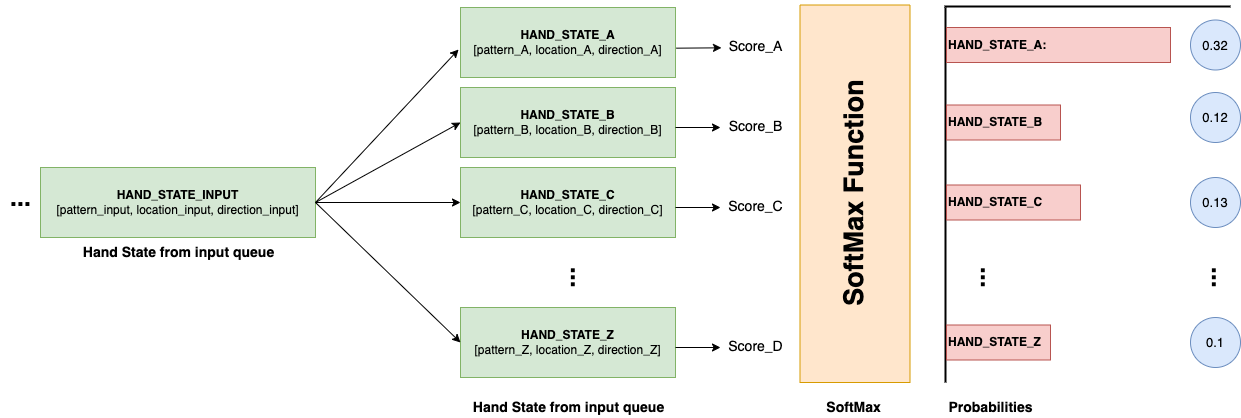
\includegraphics[width=\textwidth]{img/Chap4/Vectorization.png}
  \caption{ Vectorization }
  \label{fig:Chap4-Vectorization}
\end{figure}
% TODO: Change to Math
In the first principle, The more similarities the hand state retrieved from the queue has compared to that in the database, the higher it is scored. For example, in the database, we have a hand state as follows: 
$\begin{bmatrix}
  pattern \_ A & location \_ A & direction \_ A
\end{bmatrix}$
, and the hand state we get from the input is 
$\begin{bmatrix}
  pattern \_ A & location \_ A & direction \_ A
\end{bmatrix}$
then this hand state will be rated higher than the hand state 
$\begin{bmatrix}
  pattern \_ A & location \_ A & direction \_ B
\end{bmatrix}$
. And so on, we will, in turn, score the hand states taken from the queue.

On the second point, the minus point is evaluated based on its matching pattern with the hand states in the database. When the system recognizes patterns from the hand pattern recognition module (using the vision approach), it is likely to be wrong detected or mistaken. To resolve this problem and maximize the accuracy of the result, we put out a rule. With those patterns that are usually hard to detect, the minus point will be lower than simple ones. In short, the more complex the pattern to be recognized, the smaller the minus point is going to be.

% + Khi đánh giá các hand state, đối với trường hợp so trùng 2 pattern. Do các pattern này được nhận diện từ module hand pattern regconition (vision approach), do đó, sẽ có khả năng bị nhận diện bị sai, hoặc bị nhầm. Vì lẽ đó, để có thể đánh giá một cách chính xác và công bằng nhất có thể thì ở đây, đối với những pattern hay bị nhận diện sai, ta sẽ trừ điểm thấp và ngược lại, với những pattern đơn giản mà hệ thống lại nhận diện sai thì sẽ bị trừ điểm nhiều hơn.
      
After completing the above evaluation and scoring step, we will use a function to normalize the data (here, the authors use the softmax function) and return us a set of probabilities of the hand states in the row. Wait. We will use this set of probabilities as input for the beam search step.

\subsubsection{ Using beamsearch with CTC decode }
% TODO: Trình bày cách sử dụng beamsearch để tìm các cặp bộ 3
% TODO: Image beamsearch (get from ppt)
% TODO: Example
% TODO: Áp dụng CTC để handle một số trường hợp
% TODO: Các khó khăn gặp phải và hướng giải quyết

After passing the vectorization step, the hand states in our queue has been converted to a MxN matrix, where M is the length of the hand state's database and N is the length of queue.

By using beam search (\ref{fig:Chap4-BeamSearch}), we will get the most likely k hand state from the database. From the image below, we can imagine what happened later during beam search.

% Sau khi qua bước vectorizaion, các hand state trong hàng đợi của chúng ta
% đã được chuyển đổi thành một ma trận MxN với M là độ dài của cơ sở dữ liệu về
% các hand state và N là độ dài của hàng đợi.
      
% Bằng việc sử dụng beam search, từ sẽ thu được k hand state có khả năng nhất
% từ cơ sở dữ liệu. Từ hình ảnh bên dưới, ta có thể hình dung được những gì
% đã diễn ra sau trong quá trình thực hiện beam search

% FIXME: Insert image from ppt about matrix with beam search

\begin{figure}[H]
  \centering
  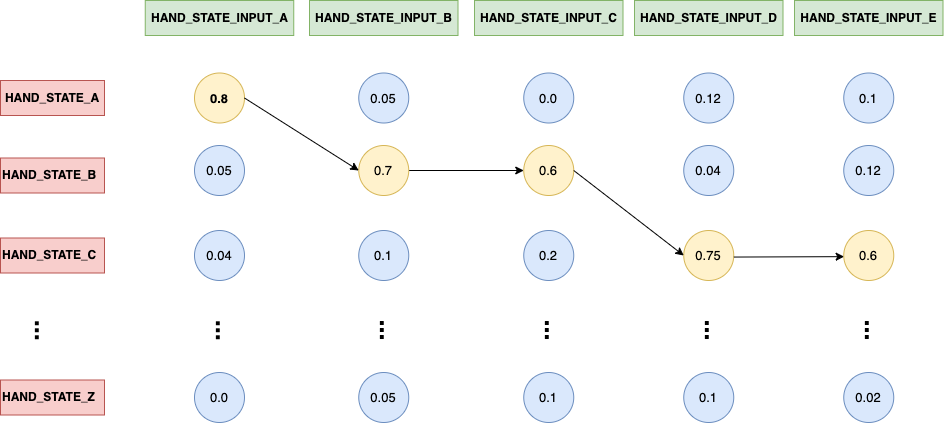
\includegraphics[width=\textwidth]{img/Chap4/BeamSearch.png}
  \caption{ Beam Search }
  \label{fig:Chap4-BeamSearch}
\end{figure}

However, as we can see that, after performing the beam search step, we will get a sequence of hand states whose length corresponds to the length of the input queue, these hand states can include duplicate hand states, or they can be wrong hand states. Therefore, we need to apply CTC algorithm to remove the hand states from infection. For the wrong hand states, in Vectorization step, we will set a threshold to discard these hand states and see it as a blank character. And after all step, after beam search CTC decode, we will get the desired result.

% Tuy nhiên, có thể thấy được rằng, sau khi thực hiện xong bước beamsearch,
% ta sẽ thu được một dãy các hand state có độ dài tương ứng với độ dài của hàng đợi
% , các hand state này có thể bao gồm những hand state bị trùng nhau, hoặc cũng có thể
% là những hand state bị sai. Do đó, ta cần áp dụng thêm CTC decode để loại bỏ các hand state
% bị trùng này. Đối với những hand state bị nhận sai từ những module trước thì ở bước Vectorization,
% ta sẽ đặt một threshold để loại bỏ những hand state này và xem như hand state đó là một ký tự rỗng (" ")
% và cuối cùng, sau khi áp dụng CTC decode vào, ta sẽ thu được kết quả mong muốn

% FIXME: Insert image about the result (get from ppt)

      
      
    \subsubsection{ Map to dictionary }
      % TODO: Cách map như thế nào

      \begin{figure}[H]
        \centering
        
\includegraphics[width=\textwidth]{img/Chap4/Result.png}
        \caption{ Map to dictionary and get word }
        \label{fig:Chap4-Result}
      \end{figure}

      % Sau khi nhận được một tập các hand state có khả năng nhất, việc còn lại là
      % chúng ta sẽ map vào cơ sở dữ liệu, như cách mà chúng ta đã làm trong mục ..., 
      % nhưng thay vì map với bộ 4 thành phần thì ở đây, ta sẽ map với input các hand state thu được
      % từ bước ... .
      % Và như thế, ta sẽ thu được từ vựng mà không cần phải dùng tới module action detection.
      After getting a set of most likely hand states, all that remains is for us to map to the database, as we did in section above, but instaed of map with 4-component set, in here, we will map with input retrieved from this previous step. And finally, we will get the word (\ref{fig:Chap4-Result}) without using the action detect module.



\subsection{Text to speech}

TODO: Add more words, like how to implement into the application

Besides displaying the translated sign language in text form, we included a text-to-speech module to know the result without looking into the screen. This module makes use of a free API provided by Google, named Text-to-Speech [4]. It converts arbitrary strings, words, and sentences into the sound of a person speaking the same things.